%%%%%%%%%%%%%%%%%%%%%%%%%%%%%%%%%%%%%%%%%%%%%%%%%%%%%%%%%%%
%                                                         %
% CHAPTER 01:                                             %
% What are quantum dots?                                  %
%                                                         %
% This file is part of a BSc Thesis Project. See the      %
% LICENSE file for more information about licensing.      %
%                                                         %
% Author:     Matteo Seclì <secli.matteo@gmail.com>       %
% A.Y.:       2014/2015                                   %
% URL:        https://github.com/matteosecli/QMC          %
%                                                         %
%%%%%%%%%%%%%%%%%%%%%%%%%%%%%%%%%%%%%%%%%%%%%%%%%%%%%%%%%%%

\graphicspath{{Mainmatter/figures/PNG/}{Mainmatter/figures/PDF/}{Mainmatter/figures/}}

\chapter{What are quantum dots?}

\section{Definition and fabrication processes}
The term ``quantum dots'' refers to finite fermion systems consisting of an artificial 3D confinement of a few electrons, that have a size of only a few hundred angstroms \citep{Reimann2002, Kastner1993}.

Such confinement is usually achieved by restricting the two-dimensional electron gas that forms at the interface between two different semiconductor materials (or heterostructure), ether laterally or vertically. Let's briefly examine these two methods.

\begin{figure}[H]
	\centering
	\begin{subfigure}[t]{0.5\textwidth}
		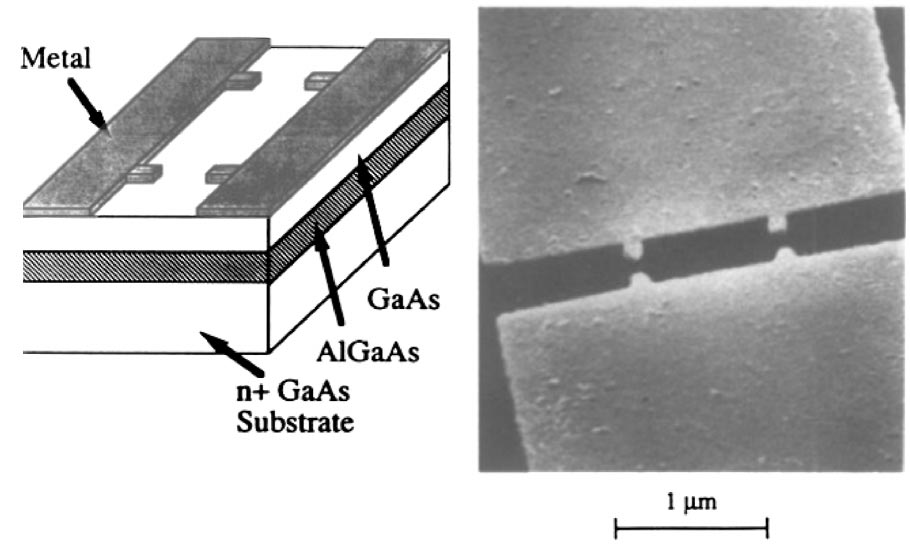
\includegraphics[width=\textwidth]{Figure_5_Reimann}
		\caption{Lateral device structure. From \cite{Meirav1990}.}
		\label{fig:Figure_5_Reimann}
    \end{subfigure}
	\begin{subfigure}[t]{0.4\textwidth}
		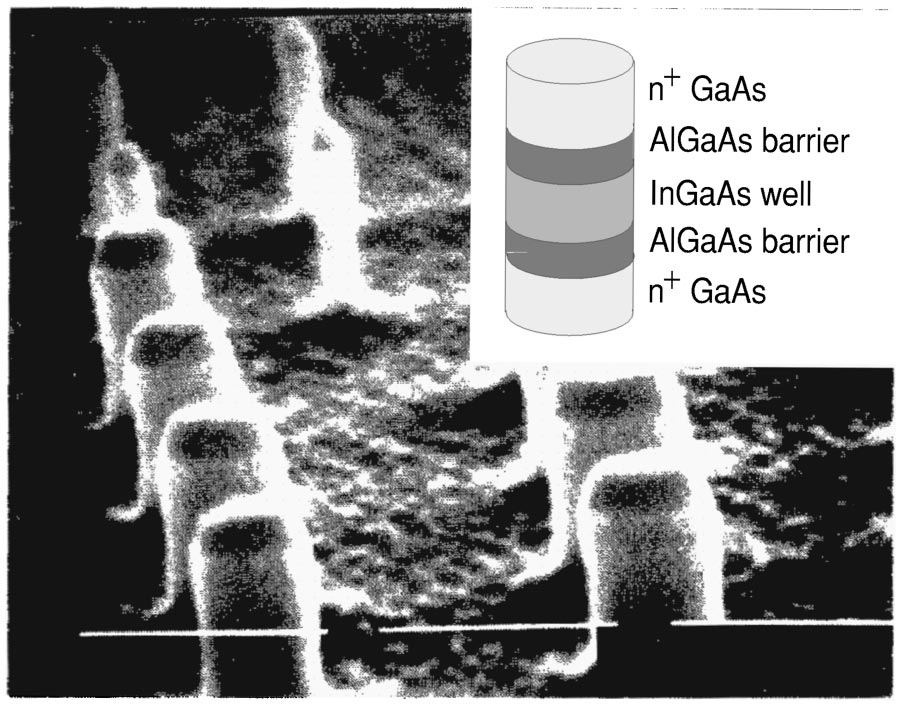
\includegraphics[width=\textwidth]{Figure_4_Reimann}
		\caption{Etched quantum dots. The white bars have a length of $\SI{0.5}{\micro\meter}$. From \cite{Reed1988}.}
		\label{fig:Figure_4_Reimann}
    \end{subfigure}
    \caption{Lateral and vertical quantum dots structures.}
	\label{fig:Figures_4-5_Reimann}
\end{figure}

The lateral confinement is obtained with a device like the one in Figure \ref{fig:Figure_5_Reimann}. The electron gas forms at the interface between GaAs and AlGaAs, and the confinement is obtained by applying a voltage to the top metal electrodes -- called gates. The entire structure is only a few $\SI{}{\micro\meter}$ thick, so the gates are created by lithographic patterning.

Another common method to fabricate quantum dots is to build heterostructure pillars by etching techniques. Some of these structures are shown in Figure \ref{fig:Figure_4_Reimann}; the electrodes are at the top and at the bottom of the pillars.

Other fabricating processes include self-growth mechanisms, in which the growth conditions determine the form of the structure (that can be pyramidal, disk shaped or lens shaped), and cleaved-edge overgrowth, that consists in two separate MBE\footnote{Molecular Beam Epitaxy} growths on a specific substrate \citep[see][]{Reimann2002}.

Although the definition of quantum dots given above is quite precise, I prefer a more immediate one: ``quantum dots are \emph{artificial atoms}''. Despite its simplicity, this definition contains a good amount of relevant information. Like natural atoms, in fact, quantum dots are made up of electrons confined in an attractive potential; and as one may guess, they show a similar shell-like structure with its relative \emph{magic numbers} -- the resemblance is striking. We begin our discussion by briefly illustrating this simple model.

\section{The shell-model}
\label{sec:shell_model}
The so-called \emph{shell-model} is a particularly convenient and simple way to treat a system of interacting particles. This model is based on the \emph{a priori} assumption that the \emph{interacting} particles can be treated as \emph{independent} particles subject to an average \emph{effective potential}. This effective potential is created by the particles themselves, but one can also add an external component to the intrinsic one. Using this simplification it's possible to find a solution for the Schr\"{o}dinger equation; the result is a certain distribution of single-particle energy levels. In many cases, this distribution it's nonuniform (look, for example, at the simple case of the infinite well) and shows a characteristic bunching of levels; these bunches are called \emph{shells}.

\begin{figure}[H]
	\centering
    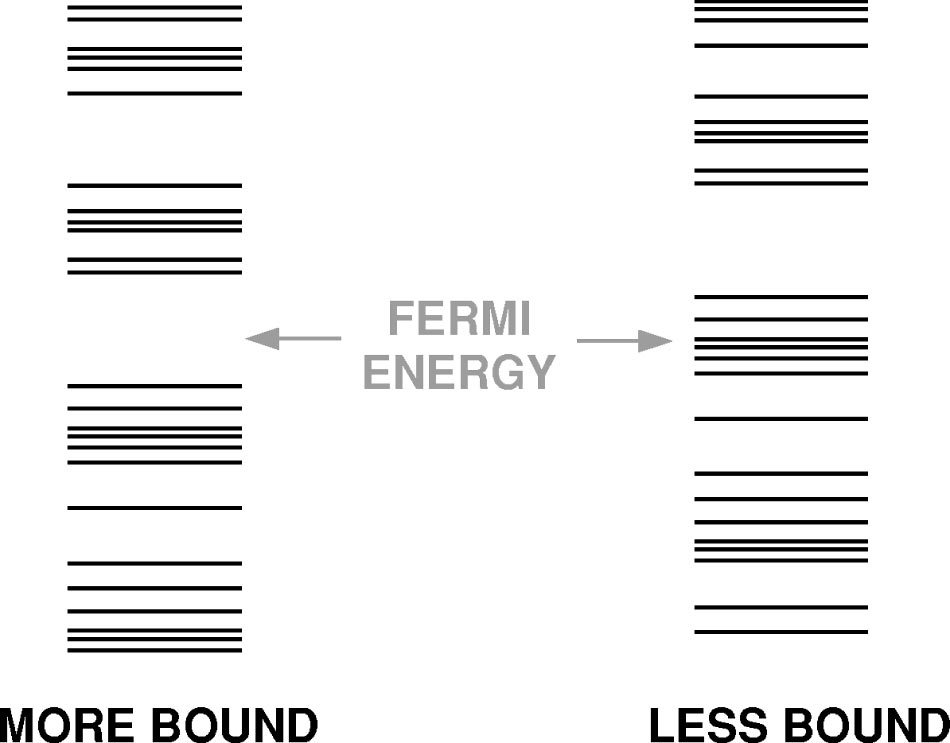
\includegraphics[width=0.5\textwidth]{Figure_1_Reimann}
    \caption{Bunching of the single-particles levels and level density at the Fermi level. From \cite{Brack1972}.}
	\label{fig:Figure_1_Reimann}
\end{figure}

It's very important to have a scheme of such energy levels, since it can immediately give information about the stability of a system: if the level bunching at the Fermi surface has a minimum, then the system is more bound. In fact, this situation corresponds to particles occupying states with a lower energy (on average), thus minimizing the total energy. In terms of the shell-model, this means that all the shells below the Fermi level are filled (see Figure \ref{fig:Figure_1_Reimann}). A situation in which the level bunching doesn't have a minimum at the Fermi surface corresponds instead in a non-filled shell. In this case the system can rearrange itself in a non-symmetric shape, in order to reach a better stability.

This has been shown e.g. for atomic nuclei by means of nuclear spectroscopy. In that case, a measurement of the \emph{quadrupole moment} can exploit the possibly non symmetric structure. As a simple example, the quadruple moment $Q$ for a single proton is
\begin{equation}
	Q = e \int \psi^*(3z^2-r^2)\psi\,d\tau,
	\label{eq:quadrupole_single_proton}
\end{equation}
where $\tau$ indicates the volume. If $|\psi|^2$ is spherically symmetric, then -- on average -- $x^2=y^2=z^2=r^2/3$, and substituting $z^2=r^2/3$ into \eqref{eq:quadrupole_single_proton} gives zero \citep[see][]{Krane1988}. So, a non-zero quadrupole moment indicates a non-spherical shape; this shape can be determined by the analysis of the angular distribution of the radiation field.

But how can these deformations give a better stability to the system in the case of non-filled shells? The answer is simple: because they minimize the energy. To show this fact, we introduce the example of a two-dimensional anisotropic harmonic oscillator confinement of fermions \citep[as in][]{Reimann2002}, in which the effective potential is 
\begin{equation}
	V(x,y) = \frac{1}{2}m^*\omega^2\left(\delta x^2 + \frac{1}{\delta}y^2\right).
\end{equation}
Here $\omega$ is the oscillator frequency, $m^*$ is the effective mass of the fermions and the deformation parameter $\delta \doteqdot \omega_x/\omega_y$ is defined such that $\omega_x=\omega\sqrt{\delta}$ and $\omega_y=\omega/\sqrt{\delta}$. This condition guarantees that the area is conserved with the deformation. By analogy with the simple harmonic oscillator, which has energy levels $E_n = \hbar\omega(n+1/2)$, the energy levels of the 2D anisotropic case are just
\begin{equation}
	E_{n_x,n_y}(\delta) = \hbar\omega\left[\sqrt{\delta}\left(n_x+\frac{1}{2}\right) + \frac{1}{\sqrt{\delta}}\left(n_y+\frac{1}{2}\right)\right].
\end{equation}
These levels are plotted against the deformation in Figure \ref{fig:Figure_2_Reimann}. For $\delta=1$ (that is the isotropic case) you see that there is a $(n+1)$-fold degeneracy, where $n=n_x+n_y=0,1,2,\ldots$ is the principal quantum number. Taking into account the spin degeneracy (that gives a factor 2), we obtain closed shells for $N=2,6,12,20,\ldots$ electrons. These numbers are called the \emph{magic numbers}. As we increase the deformation parameter, the degenerate levels split. It is useful, in this case, to look at the total energies (on the right in Figure \ref{fig:Figure_2_Reimann}); you see that now the energy levels have cups and minima that significantly change the behavior of the system for non-closed shells. In fact the energies have minima at $\delta=1$ for the closed-shell cases ($N=2,6,12$), whereas their minima are shifted to different values of $\delta$ in the open-shell cases ($N=4,8,10$). As a rough graphical estimate, for $N=4$ the minimum energy (i.e., the stablest configuration) is reached about a deformation value $\delta=2$ and for $N=10$ about $\delta=1.5$.

\begin{figure}[H]
	\centering
    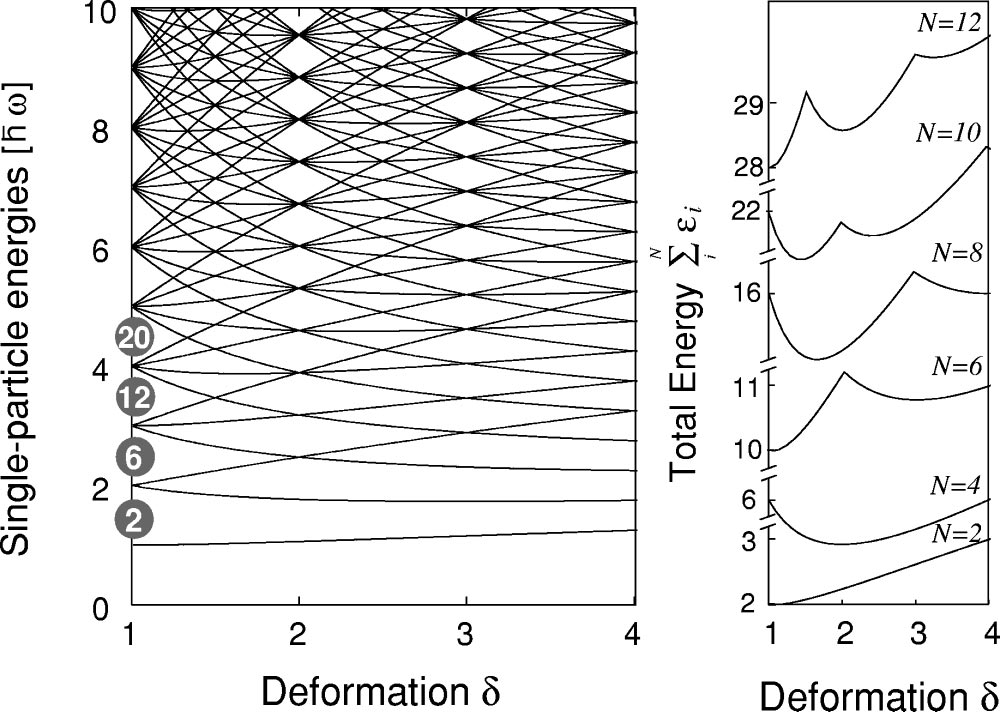
\includegraphics[width=0.65\textwidth]{Figure_2_Reimann}
    \caption{Single particle energy levels (left) and total energies (right) as a function of the deformation in a two-dimensional harmonic oscillator. From \cite{Reimann2002}.}
	\label{fig:Figure_2_Reimann}
\end{figure}

Even this simple example shows in an effective way how a deformation can guarantee a stabler configuration for non-closed shells. Further in our simulations, we will restrict only to closed-shell systems.

\section{Evidences of the shell-model}
\label{sec:shell_model_evidences}
We said before that the shell-structure seems to be a common property of finite fermion systems. Indeed, clear evidences of it had been shown for \emph{atoms}, \emph{atomic nuclei}, \emph{clusters of atoms} and \emph{quantum dots}. Let's briefly see which kind of measurements led to this results.

\begin{figure}[h]%[H]
	\centering
    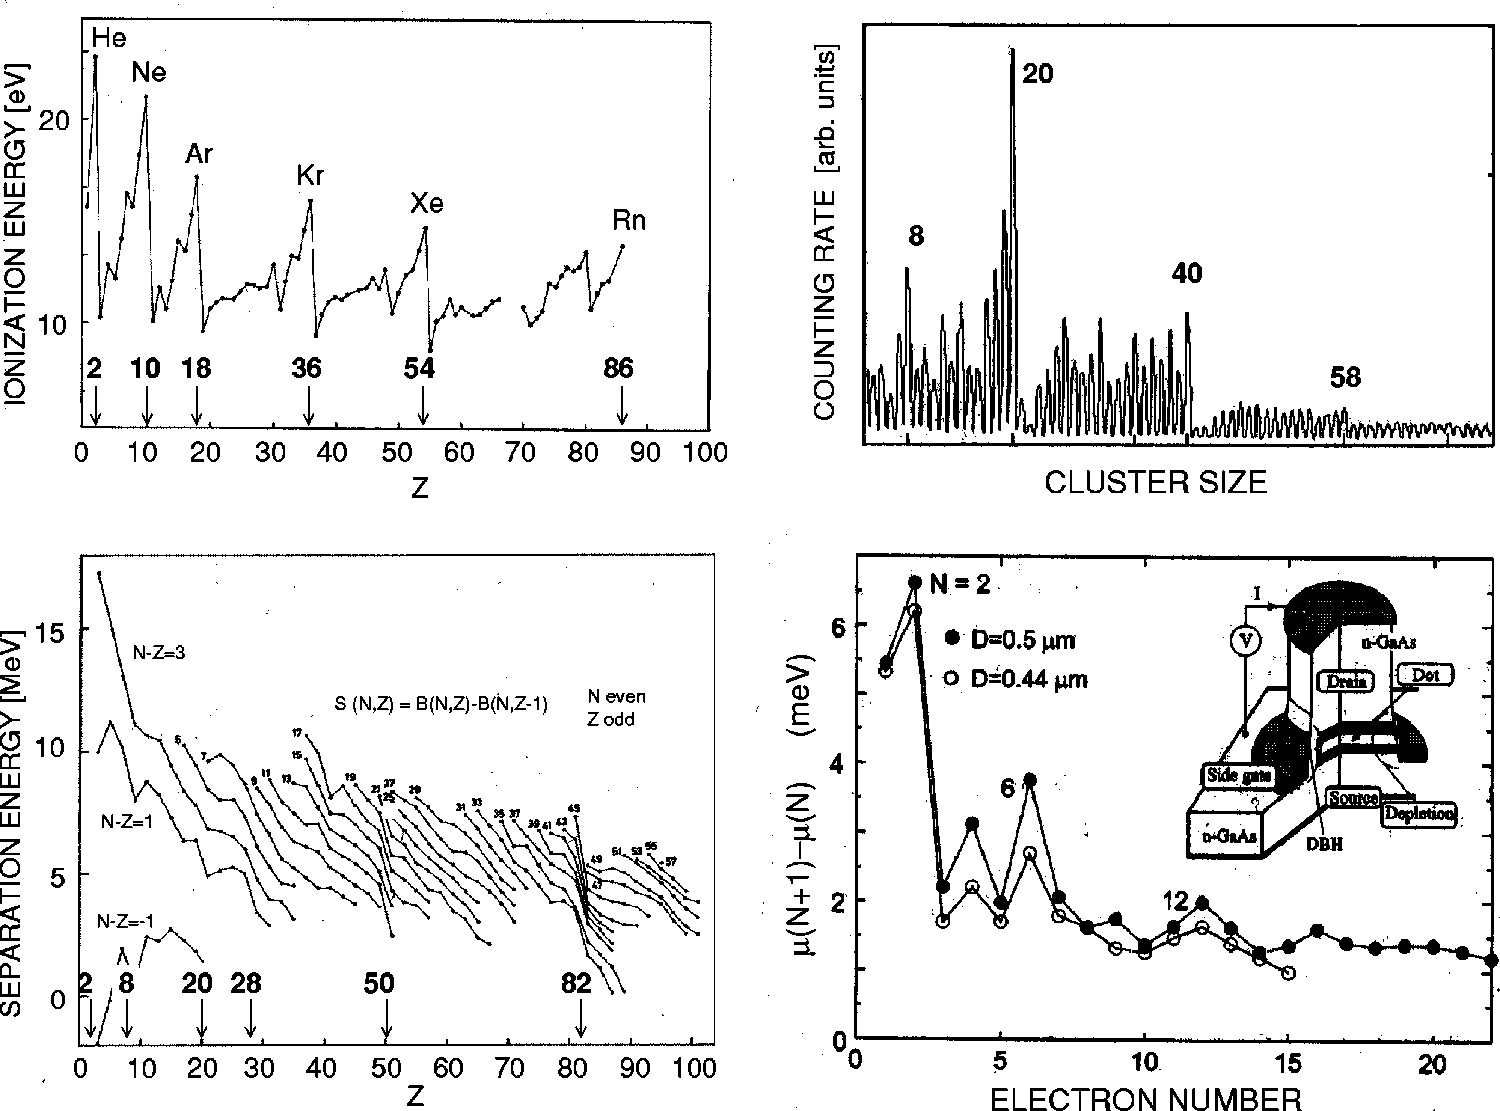
\includegraphics[width=\textwidth]{Figure_3_Reimann}
    \caption{Upper left, atomic ionization energies; lower left, separation energies of atomic nuclei; upper right, abundance spectra of metallic clusters; lower right, addition energies in a
disk-shaped quantum dot (schematized in the inset). From \cite{Reimann2002}.}
	\label{fig:Figure_3_Reimann}
\end{figure}

In the case of atoms, the shell-model is applied to the electrons ``orbiting'' around the nucleus, which is considered as an effective attractive Coulomb potential. A very natural quantity that one may think to measure in order to exploit the shell structure is the \emph{ionization energy}, that is the energy required to remove an electron from a neutral atom. In fact we have shown that electrons in a closed-shell system are more bound, which means that we expect to need more energy to remove one of it (i.e., we expect to see a higher ionization energy). Indeed this happens pretty clearly, as you see in Figure \ref{fig:Figure_3_Reimann}, upper left, showing the sequence of magic numbers $N=2,10,18,36,54,86,\ldots$.

For atomic nuclei the idea is quite the same, with the only difference that now we have to measure the energy required to remove a nucleon from the nucleus (which is called the \emph{separation energy}). The step-like behavior is also present in this case, giving the sequence of magic numbers $N=2,8,20,28,50,82,\ldots$ (Figure \ref{fig:Figure_3_Reimann}, lower left).

Atomic clusters are also an interesting case, since they show anomalies in the mass abundance spectra: for certain cluster sizes, the clusters are more stable. This behavior has been explained with the ``jellium'' theory for metallic clusters; the valence electrons are treated as trapped in a homogeneous positive-charged background (the jellium), that stems from the atomic ions. Density functional calculations showed the magic number sequence $N=2,8,20,40,58$ (see Figure \ref{fig:Figure_3_Reimann}, upper right) some years before it was discovered with experiments in the beginning of the 80's \citep[see][]{Reimann2002}.

The sequence of magic numbers for quantum dots was discovered in 1996 by using an etched pillar of semiconducting material as shown in Figure \ref{fig:Figure_3_Reimann}, lower right \citep[see also][]{Tarucha1996}. As we will see later, a quantum dot can be schematized as a one-electron transistor; measurements of the energy needed to add a single electron to a $N$-electrons quantum dot show large peaks for $N=2,6,12$ (Figure \ref{fig:Figure_3_Reimann}). Noticeably, these numbers are the same quantum numbers obtained for a two-dimensional harmonic oscillator.

\section{The Coulomb blockade model}
% Refer to it as model or effect? Found both of them.

\begin{figure}[h]%[H]
	\centering
    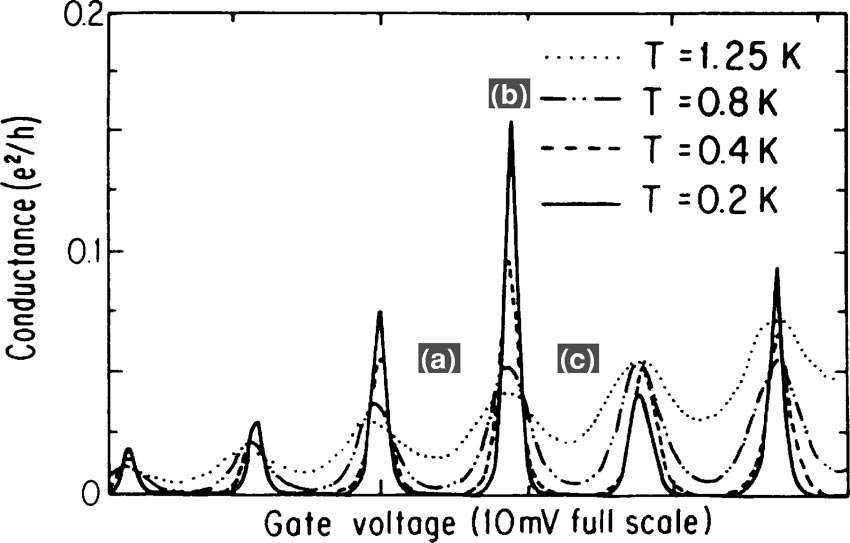
\includegraphics[width=0.60\textwidth]{Figure_6_Reimann}
    \caption{Coulomb oscillations in a lateral quantum dot. The regions (a) and (c) have a fixed number of electrons since there is a Coulomb blockade; (b) is the conductance region, where the number of electrons oscillates. Plot based on the work of \cite{Meirav1990}, by \cite{Meir1991}.}
	\label{fig:Figure_6_Reimann}
\end{figure}

The behavior of a quantum dot can be analyzed by studying its electron transport mechanism. In order to do that, the dot is connected to a circuit that provides a certain gate voltage, and its conductance is measured. A plot like the one in Figure \ref{fig:Figure_6_Reimann} is obtained; you see that there are conductance peaks at specific gate voltages, all of them evenly spaced. This behavior can be explained by the \emph{Coulomb blockade model}.

% Usage: 
\newcommand{\trcomponent}[2]
{
	\draw (#1) node[align=center] {\textnormal #2};
}

% Usage: \circlecomp{position}{text}
\newcommand{\circlecomp}[2]
{
	\draw[thick] (#1) node[draw,shape=circle,scale=0.85,align=center] {#2};
}

\newcommand{\vertcomp}[2]
{
\draw[thick] (#1) node[draw,shape=rectangle,scale=1,align=center] {\textnormal #2};
}

\begin{figure}[h]%[H]
	\centering
	\begin{circuitikz}[scale=1.1,transform shape]
		\draw (0,0) to (4,0) to (4,0.3) to[lamp,color=white,n=Vsd] ++(0,0.85);
		\draw (3.575,0.725) to (0.5,0.725) to (0.5,2.5)
			to[generic,bipoles/length=2cm,n=source] (2.5,2.5)
			to[C,l_=$C_1$,bipoles/length=1cm] (3,2.5)
			to[lamp,bipoles/length=2cm,color=white,n=dot] ++(2,0);
		\draw (4.425,0.725) to (7.5,0.725) to (7.5,2.5)
			to[generic,bipoles/length=2cm,n=drain] (5.5,2.5)
			to[C,l^=$C_2$,bipoles/length=1cm] (5,2.5);
		\draw (4,3.1) to[C,l=$C_3$,bipoles/length=1cm] (4,4.5)
			to[lamp,bipoles/length=0.9cm,color=white,n=gate] (4,5)
			to (4,5.3) to[lamp,bipoles/length=1.3cm,color=white,n=Vg] (0,5.3)
			to (0,0) node[ground] {};
		% Draw the components
		\circlecomp{Vsd}{$V_{\text{sd}}$}
		\trcomponent{source}{Source}
		\circlecomp{dot}{Dot\\$C_{\Sigma}$}
		\trcomponent{drain}{Drain}
		\vertcomp{gate}{Gate}
		\circlecomp{Vg}{$V_{\text{g}}$}
		% Draw the intrinstic indicators
		\draw[dashed] (0.4,1.5) rectangle (3.2,3.1);
		\draw[dashed] (7.6,1.5) rectangle (4.8,3.1);
		\draw[dashed] (3,3.5) rectangle (5,5.4);
	\end{circuitikz}
	\caption{Scheme of a single electron transistor. The island has index 0, the source has index 1, the drain index 2 and the gate index 3. The capacitances are meant to be intrinsic capacitances of the respective electrode (source, drain or gate). Adapted from \cite{Fasth2007}.}
	\label{fig:SET_scheme}
\end{figure}

Let's consider a \emph{single-electron transistor} device, like the one in Figure \ref{fig:SET_scheme}. This name is due to the fact that the charge on the electron island is a multiple of the elementary charge. The electron island is weakly coupled with the source and drain contacts thanks to tunnel barriers, which are thick enough to guarantee that quantum resonances dominates the electron transport mechanism.; in other words, the conductance of the tunnel must be smaller than the quantum conductance $e^2/h$ \citep[see][]{Reimann2002}. By analogy with a capacitor, in which the energy stored is $U=Q^2/2C$, one can make a first estimate of the energy stored in a dot containing $N$ particles as
\begin{equation}
	U(N) \simeq \frac{N(N-1)}{2C_{\Sigma}}.
\end{equation}
Here, the factor $(N-1)$ takes into account that each electron interacts with $N-1$ neighbors. Using this rough estimate, one can say that the energy required to add a single electron to a system already confining $N$ electrons, called the \emph{addition energy}, is
\begin{equation}
	\Delta U (N) = U(N+1)-U(N) = \frac{N(N+1)e^2}{2C_{\Sigma}} - \frac{N(N-1)e^2}{2C_{\Sigma}} = \frac{Ne^2}{C_{\Sigma}}.
\end{equation}
You see that, for successive $N$'s, the energy values are separated by the so-called \emph{charging energy}, $e^2/C_{\Sigma}$, which is constant. At low enough temperatures and bias voltages, the charging energy might be larger than the thermal energy ($e^2/C_{\Sigma} \gg k_BT$), thus preventing the electrons from tunneling the barriers. In this case transport is blocked, and this effect is called the \emph{Coulomb blockade}.

Let's now analyze the same situation in a more precise way \citep[adapted from][]{Fasth2007}. If we label the dot with the index $i=0$, the source with 1, the drain with 2 and the gate with 3, the induced charge $\tilde{Q}_i$ on each of the electrodes can be written as
\begin{equation}
	\tilde{Q}_i = \sum_{j=0}^{n}C_{ij}V_j,
\end{equation}
where $C_{ij}$ is the capacitance matrix, $V_j$ is the potential on the $j$'th element, and $n$ will be in general larger than 3 because of additional gate electrodes. If we refer to the dot ($i=0$), we can then write
\begin{equation}
	\tilde{Q}_0 = \sum_{j=0}^{n}C_{0j}V_j = C_{00}V_0 + \sum_{j=1}^{n}C_{0j}V_j,
\end{equation}
from which
\begin{equation}
	V_0 = \frac{1}{C_{00}}\left(\tilde{Q}_0 - \sum_{j=1}^{n}C_{0j}V_j\right).
	\label{eq:V0_vs_Q0tilde}
\end{equation}
In general, the induced charge $\tilde{Q}_0$ will be not equal to the measured one, $Q_0$, because of the presence of a background charge $Q_{\text{bg}}$ (that can be measured if all the potentials are set to zero). This means that $\tilde{Q}_0 = Q_0 - Q_{\text{bg}}$. Moreover, $C_{\Sigma} \equiv C_{00}$ by definition, and we can find an expression for it using the charge neutrality condition $\sum_{j=0}^{n}C_{0j}=0$, which implies $C_{\Sigma} \equiv C_{00} = -\sum_{j=1}^{n}C_{0j}$. Using these two facts, we can rewrite equation \eqref{eq:V0_vs_Q0tilde} as
\begin{equation}
	V_0(Q_0) = \frac{1}{C_{\Sigma}}\left(Q_0 - Q_{\text{bg}} - \sum_{j=1}^{n}C_{0j}V_j\right).
	\label{eq:V0_vs_Q0}
\end{equation}

At this point, we can calculate the energy $U(N)$ stored in a dot with $N$ electrons by performing an integration:
\begin{equation}
	U(N) = \int_{0}^{-eN}V_0(Q_0)\,dQ_0 = \frac{e^2N^2}{2C_{\Sigma}} + eN\left( \frac{Q_{\text{bg}}}{C_{\Sigma}} + \sum_{j=1}^{n}\frac{C_{0j}}{C_{\Sigma}}V_j \right).
\end{equation}

Using this expression, we can finally calculate the addition energy as
\begin{equation}
	\Delta U (N) = U(N+1)-U(N) = \frac{e^2}{C_{\Sigma}}\left(N+\frac{1}{2}\right) + e\left( \frac{Q_{\text{bg}}}{C_{\Sigma}} + \sum_{j=1}^{n}\frac{C_{0j}}{C_{\Sigma}}V_j \right).
\end{equation}
You see that, for small temperatures and bias voltages, we can approximate $\Delta U (N) \simeq e^2N/C$ as we found previously by a rough estimate.

This calculation still lacks the fact that, in such a small device, quantization effects are also important and should be considered. A simple model that combines the Coulomb blockade effect and the quantum effects is the \emph{constant interaction model}.

\section{The constant interaction model}
The basis assumption of the constant interaction model is that the total energy $E(N)$ of the electron island is the sum of the single-particle energies and the electrostatic energy $U(N)$:
\begin{equation}
	E(N) = \sum_{i=1}^{N}\epsilon_i + U(N) = \sum_{i=1}^{N}\epsilon_i + \frac{e^2N^2}{2C_{\Sigma}} + eN\left( \frac{Q_{\text{bg}}}{C_{\Sigma}} + \sum_{j=1}^{n}\frac{C_{0j}}{C_{\Sigma}}V_j \right).
\end{equation}
From this expression we can calculate the \emph{electrochemical potential} $\mu_N$, that is defined as the necessary energy to add the $N$-th electron to a conductor, as
\begin{equation}
	\mu_N 
	= E(N) - E(N-1) 
	=  \epsilon_N + \frac{e^2}{C_{\Sigma}}\left(N-\frac{1}{2}\right) + e\left( \frac{Q_{\text{bg}}}{C_{\Sigma}} - \sum_{j=1}^{n}\alpha_jV_j \right),
	\label{eq:electrochemical_potential}
\end{equation}
where $\alpha_j$, defined as
\begin{equation}
	\alpha_j \doteqdot - \frac{C_{0j}}{C_{\Sigma}},
\end{equation}
is called the \emph{lever arm} of the gate $j$ and is always positive. Experiments show that the lever arm changes in a significant way only for very large gate voltage variations; so, in most cases the lever arm can be considered constant \citep{Fasth2007}. This implies that the relation between the electrochemical potential and the gate voltage in equation \eqref{eq:electrochemical_potential} is linear; an increase in the gate voltage reflects in a decrease of the electrochemical potential, and vice-versa.

One can also calculate the spacing between different $\mu_N$'s, that is
\begin{equation}
	\mu_{N+1}-\mu_N 
	= \epsilon_{N+1} - \epsilon_{N} + \frac{e^2}{C_{\Sigma}}
	= \Delta_{N+1} + \frac{e^2}{C_{\Sigma}},
\end{equation}
where $\Delta_{N+1}\doteqdot \epsilon_{N+1} - \epsilon_{N}$ is the spacing between two successive single-particles energy levels. You immediately note that, when $\Delta_{N+1} \ll k_BT \ll e^2/C_{\Sigma}$, the quantum effects can be neglected and the Coulomb blockade oscillations are periodic in $e^2/C_{\Sigma}$ \citep{Reimann2002}.

\begin{figure}
	\centering
	\begin{subfigure}[t]{0.45\textwidth}
		\newcommand{\ThickBorder}{(0,3) -- (2.8,3) -- (2.8,9) -- (3.2,9) -- (3.2,1) -- (5.8,1) -- (5.8,8.6) -- (6.2,8.6) -- (6.2,2.5) -- (9,2.5)}
		\begin{tikzpicture}[scale=0.8]%every node/.style={transform shape}
			\tikzset{>=latex}
			
			% Fill dark region
			\fill[draw=none,fill=black!40!white]
				(0,0) -- \ThickBorder -- (9,0) -- cycle;
				
			%Fill light regions
			\fill[draw=none,fill=black!10!white]
				(0,3) -- (2.8,3) -- (2.8,6) -- (0,6) -- cycle;
			\fill[draw=none,fill=black!10!white]
				(3.2,1) -- (5.8,1) -- (5.8,5) -- (3.2,5) -- cycle;
			\fill[draw=none,fill=black!10!white]
				(6.2,2.5) -- (9,2.5) -- (9,5.6) -- (6.2,5.6) -- cycle;
				
			% Draw thick border
			\draw[thick] \ThickBorder;
			
			% Draw source potential
			\draw[very thick] (0,6) -- (2.8,6) node[midway,above] {$\mu_S$};
			
			% Draw dot potential
			\draw[very thick] (3.2,5) -- (5.8,5) node[midway,above] {$\mu_N$};
			\draw[very thick, dashed] (3.2,7.2) -- (5.8,7.2) node[midway,above] {$\mu_{N+1}$};
			 
			% Draw drain potential
			\draw[very thick] (6.2,5.6) -- (9,5.6) node[midway,above] {$\mu_D$};
			
			% Draw units
			\draw[<->, thick] (5,5) -- (5,7.2)
				node[midway,fill=white,text=black,xshift=-0.4cm,yshift=0.05cm]
				{\scriptsize $\dfrac{e^2}{C_{\Sigma}} + \Delta_{N+1}$};
			\draw[<->, thick] (6.4,1) -- (6.4,2.5)
				node[midway,fill=black!40!white,text=black,xshift=+0.45cm]
				{\scriptsize $U_{N+1}(V_G)$};
			 
		\end{tikzpicture}	
		\caption{$\mu_N<\mu_D$: the transport is blocked due to the Coulomb blockade. The number of electrons inside the dot is $N$.}
		\label{fig:SET_mu_potential_stage1}
	\end{subfigure}
	$\qquad$
	\begin{subfigure}[t]{0.45\textwidth}
		\newcommand{\ThickBorderUp}{(0,3) -- (2.8,3) -- (2.8,9) -- (3.2,9) -- (3.2,1.8) -- (5.8,1.8) -- (5.8,8.5) -- (6.2,8.5) -- (6.2,2.5) -- (9,2.5)}
		\begin{tikzpicture}[scale=0.8]%every node/.style={transform shape}
			\tikzset{>=latex}
			
			% Fill dark region
			\fill[draw=none,fill=black!40!white]
				(0,0) -- \ThickBorderUp -- (9,0) -- cycle;
				
			%Fill light regions
			\fill[draw=none,fill=black!10!white]
				(0,3) -- (2.8,3) -- (2.8,6) -- (0,6) -- cycle;
			\fill[draw=none,fill=black!10!white]
				(3.2,1.8) -- (5.8,1.8) -- (5.8,3.6) -- (3.2,3.6) -- cycle;
			\fill[draw=none,pattern=north east lines,pattern color=black!10!white]
				(3.2,3.6) -- (5.8,3.6) -- (5.8,5.8) -- (3.2,5.8) -- cycle;
			\fill[draw=none,fill=black!10!white]
				(6.2,2.5) -- (9,2.5) -- (9,5.6) -- (6.2,5.6) -- cycle;
				
			% Draw thick border
			\draw[thick] \ThickBorderUp;
			
			% Draw source potential
			\draw[very thick] (0,6) -- (2.8,6) node[midway,above] {$\mu_S$};
			
			% Draw dot potential
			\draw[very thick] (3.2,5.8) -- (5.8,5.8) node[midway,above] {$\mu_N$};
			\draw[very thick] (3.2,3.6) -- (5.8,3.6) node[midway,above] {$\mu_{N-1}$};
			 
			% Draw drain potential
			\draw[very thick] (6.2,5.6) -- (9,5.6) node[midway,above] {$\mu_D$};
			
			% Draw units
			\draw[<->, thick] (6.4,1.8) -- (6.4,2.5)
				node[midway,fill=black!40!white,text=black,xshift=+0.80cm,yshift=-0.02cm]
				{\scriptsize $U_{N}(V_G)$};
			 
		\end{tikzpicture}	
		\caption{$\mu_S \gtrsim \mu_N \gtrsim \mu_D$: one electron can tunnel the barrier. The number of electrons inside the dot varies from $N-1$ to $N$. This configuration is obtain by lowering $V_G$, in order to increase $\mu_N$.}
		\label{fig:SET_mu_potential_stage2}	
	\end{subfigure}
	\begin{subfigure}[t]{0.45\textwidth}
		\newcommand{\ThickBorderUp}{(0,3) -- (2.8,3) -- (2.8,9) -- (3.2,9) -- (3.2,2.4) -- (5.8,2.4) -- (5.8,8.5) -- (6.2,8.5) -- (6.2,2.5) -- (9,2.5)}
		\begin{tikzpicture}[scale=0.8]%every node/.style={transform shape}
			\tikzset{>=latex}
			
			% Fill dark region
			\fill[draw=none,fill=black!40!white]
				(0,0) -- \ThickBorderUp -- (9,0) -- cycle;
				
			%Fill light regions
			\fill[draw=none,fill=black!10!white]
				(0,3) -- (2.8,3) -- (2.8,6) -- (0,6) -- cycle;
			\fill[draw=none,fill=black!10!white]
				(3.2,2.4) -- (5.8,2.4) -- (5.8,4.2) -- (3.2,4.2) -- cycle;
			\fill[draw=none,fill=black!10!white]
				(6.2,2.5) -- (9,2.5) -- (9,5.6) -- (6.2,5.6) -- cycle;
				
			% Draw thick border
			\draw[thick] \ThickBorderUp;
			
			% Draw source potential
			\draw[very thick] (0,6) -- (2.8,6) node[midway,above] {$\mu_S$};
			
			% Draw dot potential
			\draw[very thick, dashed] (3.2,6.4) -- (5.8,6.4) node[midway,above] {$\mu_N$};
			\draw[very thick] (3.2,4.2) -- (5.8,4.2) node[midway,above] {$\mu_{N-1}$};
			 
			% Draw drain potential
			\draw[very thick] (6.2,5.6) -- (9,5.6) node[midway,above] {$\mu_D$};
			 
		\end{tikzpicture}	
		\caption{$\mu_N>\mu_S$: the transport is blocked again due to the Coulomb blockade. The number of electrons inside the dot is $N-1$. This situation is obtained by further lowering $V_G$.}
		\label{fig:SET_mu_potential_stage3}
		\end{subfigure}
	\caption{Energy diagram of a quantum dot. The sequence of images illustrates the transport process of the electrons \citep[adapted from][]{Fasth2007}.}
	\label{fig:SET_mu_potential}
\end{figure}

Using this information, we can now analyze the transport mechanism in a quantum dot. Let's consider -- as explained before -- the low-temperature, low-bias voltage case ($eV_{\text{bias}},k_BT \ll e^2/C_{\Sigma}$). Let's also suppose that, initially, the electrochemical potential inside the dot -- $\mu_N$ -- is lower than the electrochemical potential of the drain -- $\mu_D$: the transport is blocked due to the Coulomb blockade effect (Figure \ref{fig:SET_mu_potential_stage1}). Now, we can decrease the gate voltage: the overall effect, as you can see from equation \eqref{eq:electrochemical_potential} and from our previous considerations, is that we have a linear increase in $\mu_N$ wrt the gate voltage. Eventually, $\mu_N$ will align to $\mu_D$ ($\mu_N = \mu_D$), which means that an electron can leave the dot. At the same time, if $\mu_S \gtrsim \mu_D$, an electron from $\mu_S$ can enter the dot; the overall effect is that the number of the electrons inside the dot oscillates between $N$ and $N-1$, and an electric current flows though the dot from the drain to the source (Figure \ref{fig:SET_mu_potential_stage2}). In terms of the conductance, this corresponds in a peak. If we keep lowering the gate voltage -- i.e., increasing $\mu_N$ -- until $\mu_N > \mu_S$, then the dot is left with only $N-1$ electrons. Now, the level to consider is $\mu_{N-1}$: you see that it's far below $\mu_D$, so the current is blocked again (see Figure \ref{fig:SET_mu_potential_stage3}).

This qualitative analysis also permits to find the gate voltage values for which we have peaks in the conductance. The peak condition, in fact, is $\mu_S\approx\mu_N\approx\mu_D$; inserting this condition in \eqref{eq:electrochemical_potential} and solving for $V_3$ (the index 3 indicates the gate, so we will replace the subscript with ``G'' for simplicity) gives
\begin{align}
	V_G^{(N)}
	&\approx \frac{1}{e\alpha_G}\left[ \epsilon_N + \frac{e^2}{C_{\Sigma}}\left(N-\frac{1}{2}\right) + \frac{eQ_{\text{bg}}}{C_{\Sigma}} - \mu_S - e\sum_{j=4}^{n}\alpha_jV_j - e\sum_{j=1}^{2}\alpha_jV_j \right] \\
	&\approx \frac{1}{e\alpha_G}\left[ \epsilon_N + \frac{e^2}{C_{\Sigma}}\left(N-\frac{1}{2}\right) + \frac{eQ_{\text{bg}}}{C_{\Sigma}} - \mu_S - e\sum_{j=4}^{n}\alpha_jV_j \right]
\end{align}
where the last term has been dropped because we are in the small-bias voltage case. The gate-voltage spacing between two peaks is finally found as (converted to energy)
\begin{align}
	e\Delta V_G(N) 
	&= e\Big[V_G^{(N)}-V_G^{(N-1)}\Big] \\
	&= \frac{1}{\alpha_G}\left( \epsilon_N - \epsilon_{N-1} + \frac{e^2}{C_{\Sigma}} \right) \\
	&= \frac{1}{\alpha_G}\left( \Delta_N + \frac{e^2}{C_{\Sigma}} \right).
	\label{eq:DeltaVG_N_Vb0}
\end{align}

As we already noticed before, for a lateral structure we can neglect the single-particle levels spacing (because the structure itself is quite large); this is not true for a vertical quantum dots structure, that has far smaller dimensions (as you can see in Figure \ref{fig:Figures_4-5_Reimann}). In that case the space quantization is evident and the conductance peaks are not evenly spaced, as you can see in Figure \ref{fig:Figure_10_Reimann}. It's also very nice that, by simply subtracting the quantity $1 / \alpha_G (e^2 / C_{\Sigma})$ from the spacing of two successive peaks, we can reconstruct the spectrum of the dot.

\begin{figure}[h]%[H]
	\centering
    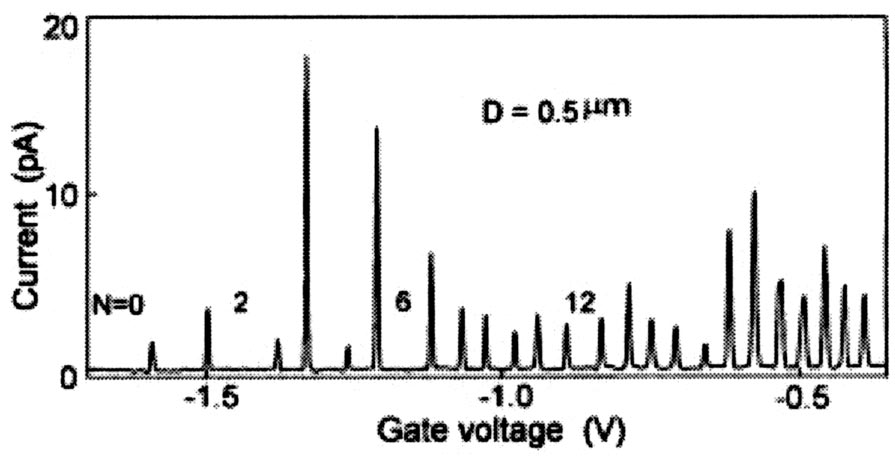
\includegraphics[width=0.55\textwidth]{Figure_10_Reimann}
    \caption{Coulomb oscillations in a vertical quantum dot. Here, $D$ is an estimate for the dot diameter. From \cite{Tarucha1996}.}
	\label{fig:Figure_10_Reimann}
\end{figure}

Finally, we briefly discuss the case in which the bias voltage cannot be neglected. Let's put us in the simple case of a symmetric bias voltage between the drain and the source, i.e.
\begin{equation}
	\begin{cases}
		V_S = V_{\text{bias}}/2 \\
		V_D = -V_{\text{bias}}/2
	\end{cases}
\end{equation}
which means that
\begin{equation}
	\begin{cases}
		\mu_S = \mu_0 + eV_{\text{bias}}/2 \\
		\mu_D = \mu_0 - eV_{\text{bias}}/2
	\end{cases}
\end{equation}
Here, $\mu_0$ is the electrochemical potential of both drain and source when the bias voltage is zero.

We showed before that the dot does not conduct for
\begin{equation}
	 \mu_N < \mu_D < \mu_S < \mu_{N+1}, \qquad V_{\text{bias}} > 0,
\end{equation}
and
\begin{equation}
	 \mu_N < \mu_S < \mu_D < \mu_{N+1}, \qquad V_{\text{bias}} < 0,
\end{equation}
so the borders of the Coulomb blockade region are defined by
\begin{equation}
	\mu_N = 
	\begin{cases}
		\mu_D = \mu_0 - eV_{\text{bias}}/2, & V_{\text{bias}} > 0 \\
		\mu_S = \mu_0 + eV_{\text{bias}}/2, & V_{\text{bias}} < 0
	\end{cases}
\end{equation}
and
\begin{equation}
	\mu_{N+1} = 
	\begin{cases}
		\mu_S = \mu_0 + eV_{\text{bias}}/2, & V_{\text{bias}} > 0 \\
		\mu_D = \mu_0 - eV_{\text{bias}}/2, & V_{\text{bias}} < 0
	\end{cases}
\end{equation}
Substituting these values for $\mu_N$, $V_S$ and $V_D$ in \eqref{eq:electrochemical_potential}, we finally find that the borders of the Coulomb blockade are the straight lines of equations
\begin{dmath}
	V_G^{(N)}(V_{\text{bias}})
	= \frac{1}{e\alpha_G}\left[ \epsilon_N + \frac{e^2}{C_{\Sigma}}\left(N-\frac{1}{2}\right) \\
	+ \frac{eQ_{\text{bg}}}{C_{\Sigma}} - \mu_0 - e(\alpha_S-\alpha_D-1)\frac{V_{\text{bias}}}{2} - e\sum_{j=4}^{n}\alpha_jV_j \right]
	\label{eq:VG_N}
\end{dmath}
and
\begin{dmath}
	V_G^{(N+1)}(V_{\text{bias}})
	= \frac{1}{e\alpha_G}\left[ \epsilon_{N+1} + \frac{e^2}{C_{\Sigma}}\left(N+\frac{1}{2}\right) \\
	+ \frac{eQ_{\text{bg}}}{C_{\Sigma}} - \mu_0 - e(\alpha_S-\alpha_D+1)\frac{V_{\text{bias}}}{2} - e\sum_{j=4}^{n}\alpha_jV_j \right]
	\label{eq:VG_N+1}
\end{dmath}
for $V_{\text{bias}}>0$. The case $V_{\text{bias}}<0$ is handled similarly.

By equating \eqref{eq:VG_N} and \eqref{eq:VG_N+1} we find that these two lines cross at $eV_{\text{bias}} = \Delta_{N+1} + e^2/C_{\Sigma}$, where $\Delta_{N+1}=\varepsilon_{N+1}-\varepsilon_{N}$ as usual. For $V_{\text{bias}}=0$, instead, we find that the spacing between $V_G^{(N)}$ and $V_G^{(N+1)}$ is $(\Delta_{N+1} + e^2/C_{\Sigma})/\alpha_G$ as we found previously for a negligible $V_{\text{bias}}$, equation \eqref{eq:DeltaVG_N_Vb0}. The situation is schematically pictured in Figure \ref{fig:diamond_regions}.

\begin{figure}[h]%[H]
	\centering
	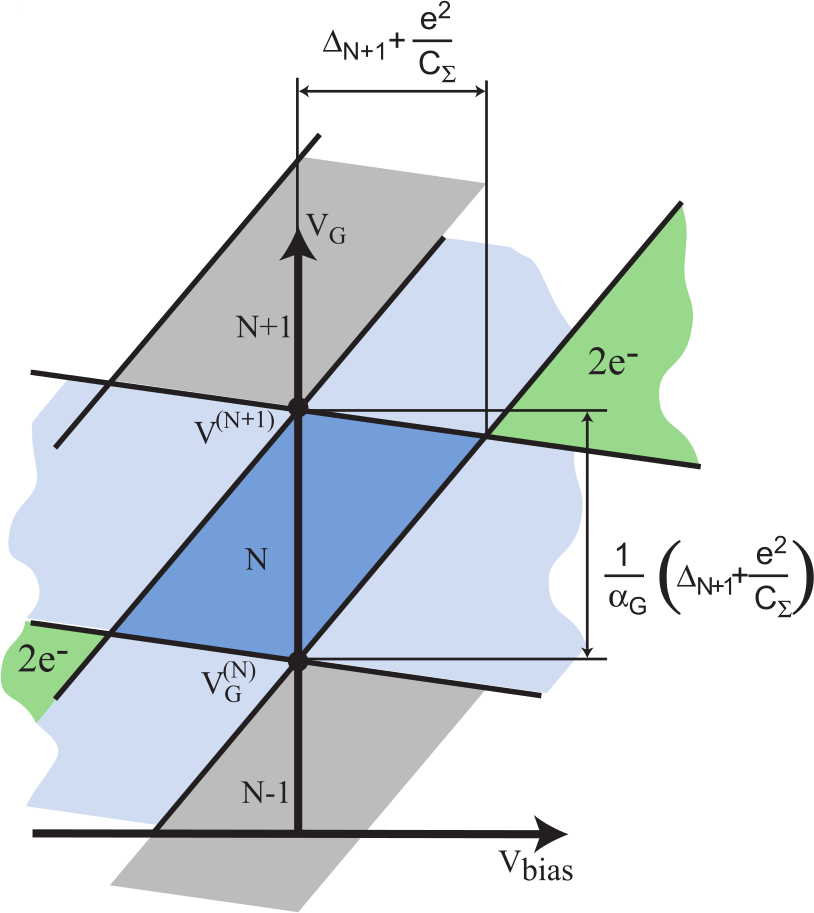
\includegraphics[width=0.5\textwidth]{diamond_regions}
	\caption{Coulomb blockade diamonds (gray and dark blue regions). In the dark blue region, the probability of finding $N$ electrons in the dot is $1$ (stable configuration); in the light blue regions, the probability varies from 0 to 1 and the electron number can change by one. In the green region, the bias voltage is so high that eventually $eV_{\text{bias}} > e^2/C_{\Sigma}$; due to this fact, two electrons can tunnel at the same time. From \cite{Fasth2007}.}
	\label{fig:diamond_regions}
\end{figure}

The diamond-shaped structure shown in Figure \ref{fig:diamond_regions} have been shown in differential conductance measurements like the one shown in Figure \ref{fig:Figure_8_Reimann}. A 3D elaboration of the data obtained from this kind of experiment -- that clarifies the ideas a little bit -- is shown in Figure \ref{fig:diff_conductance_3D}.

\begin{figure}[H]
	\centering
	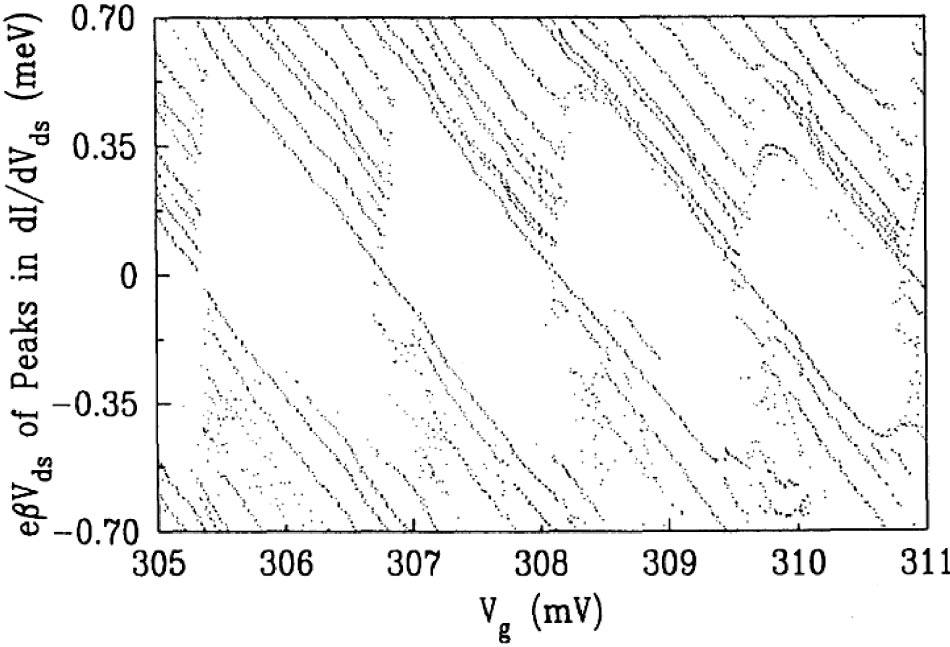
\includegraphics[width=0.6\textwidth]{Figure_8_Reimann}
	\caption{Peaks in the differential conductance $\partial I/\partial V_{\text{sd}}$ (showed as solid lines) of a lateral quantum dot, as a function of $V_{\text{sd}}$ and $V_{\text{g}}$. The white regions are the Coulomb blockade regions; between successive regions, the number of electrons in the dot is increased by one. From \cite{Reimann2002}.}
	\label{fig:Figure_8_Reimann}
\end{figure}

\begin{figure}[H]
	\centering
	\def\svgwidth{0.8\textwidth}
	\input{Mainmatter/figures/diff_conductance_3D.pdf_tex}
	\caption{Differential conductance $\partial I/\partial V_{\text{sd}}$ in a nanowire, plotted against $V_{\text{sd}}$ and $V_{\text{g}}$. Green and red indicate positive values; blue means close to zero, whereas pink stands for negative. From \cite{Weinmann1994}.}
	\label{fig:diff_conductance_3D}
\end{figure}

\section{The parabolic confinement}
In our simulation, we will model the confining (single-particle) potential as a \emph{two-dimensional harmonic trap}. This form for the confining potential is widely accepted as a standard for both exact and effective-field calculations, and is the result of experimental observations and numerical calculations.

The basis for this assumption can be found in the work of \cite{Kumar1990}. They performed numerical calculations on the Poisson and Schr\"{o}dinger equations to obtain the electron states in a GaAs/AlGaAs quantum dot -- like the one sketched in Figure \ref{fig:Figure_5_Reimann}. The calculations were done in the Hartree approximation. The results were quite interesting, as you can see in Figure \ref{fig:Figure_2_Kumar}; despite the square shape of the GaAs cap, the contours of the effective confinement potential were circular.

\begin{figure}[h]%[H]
	\centering
	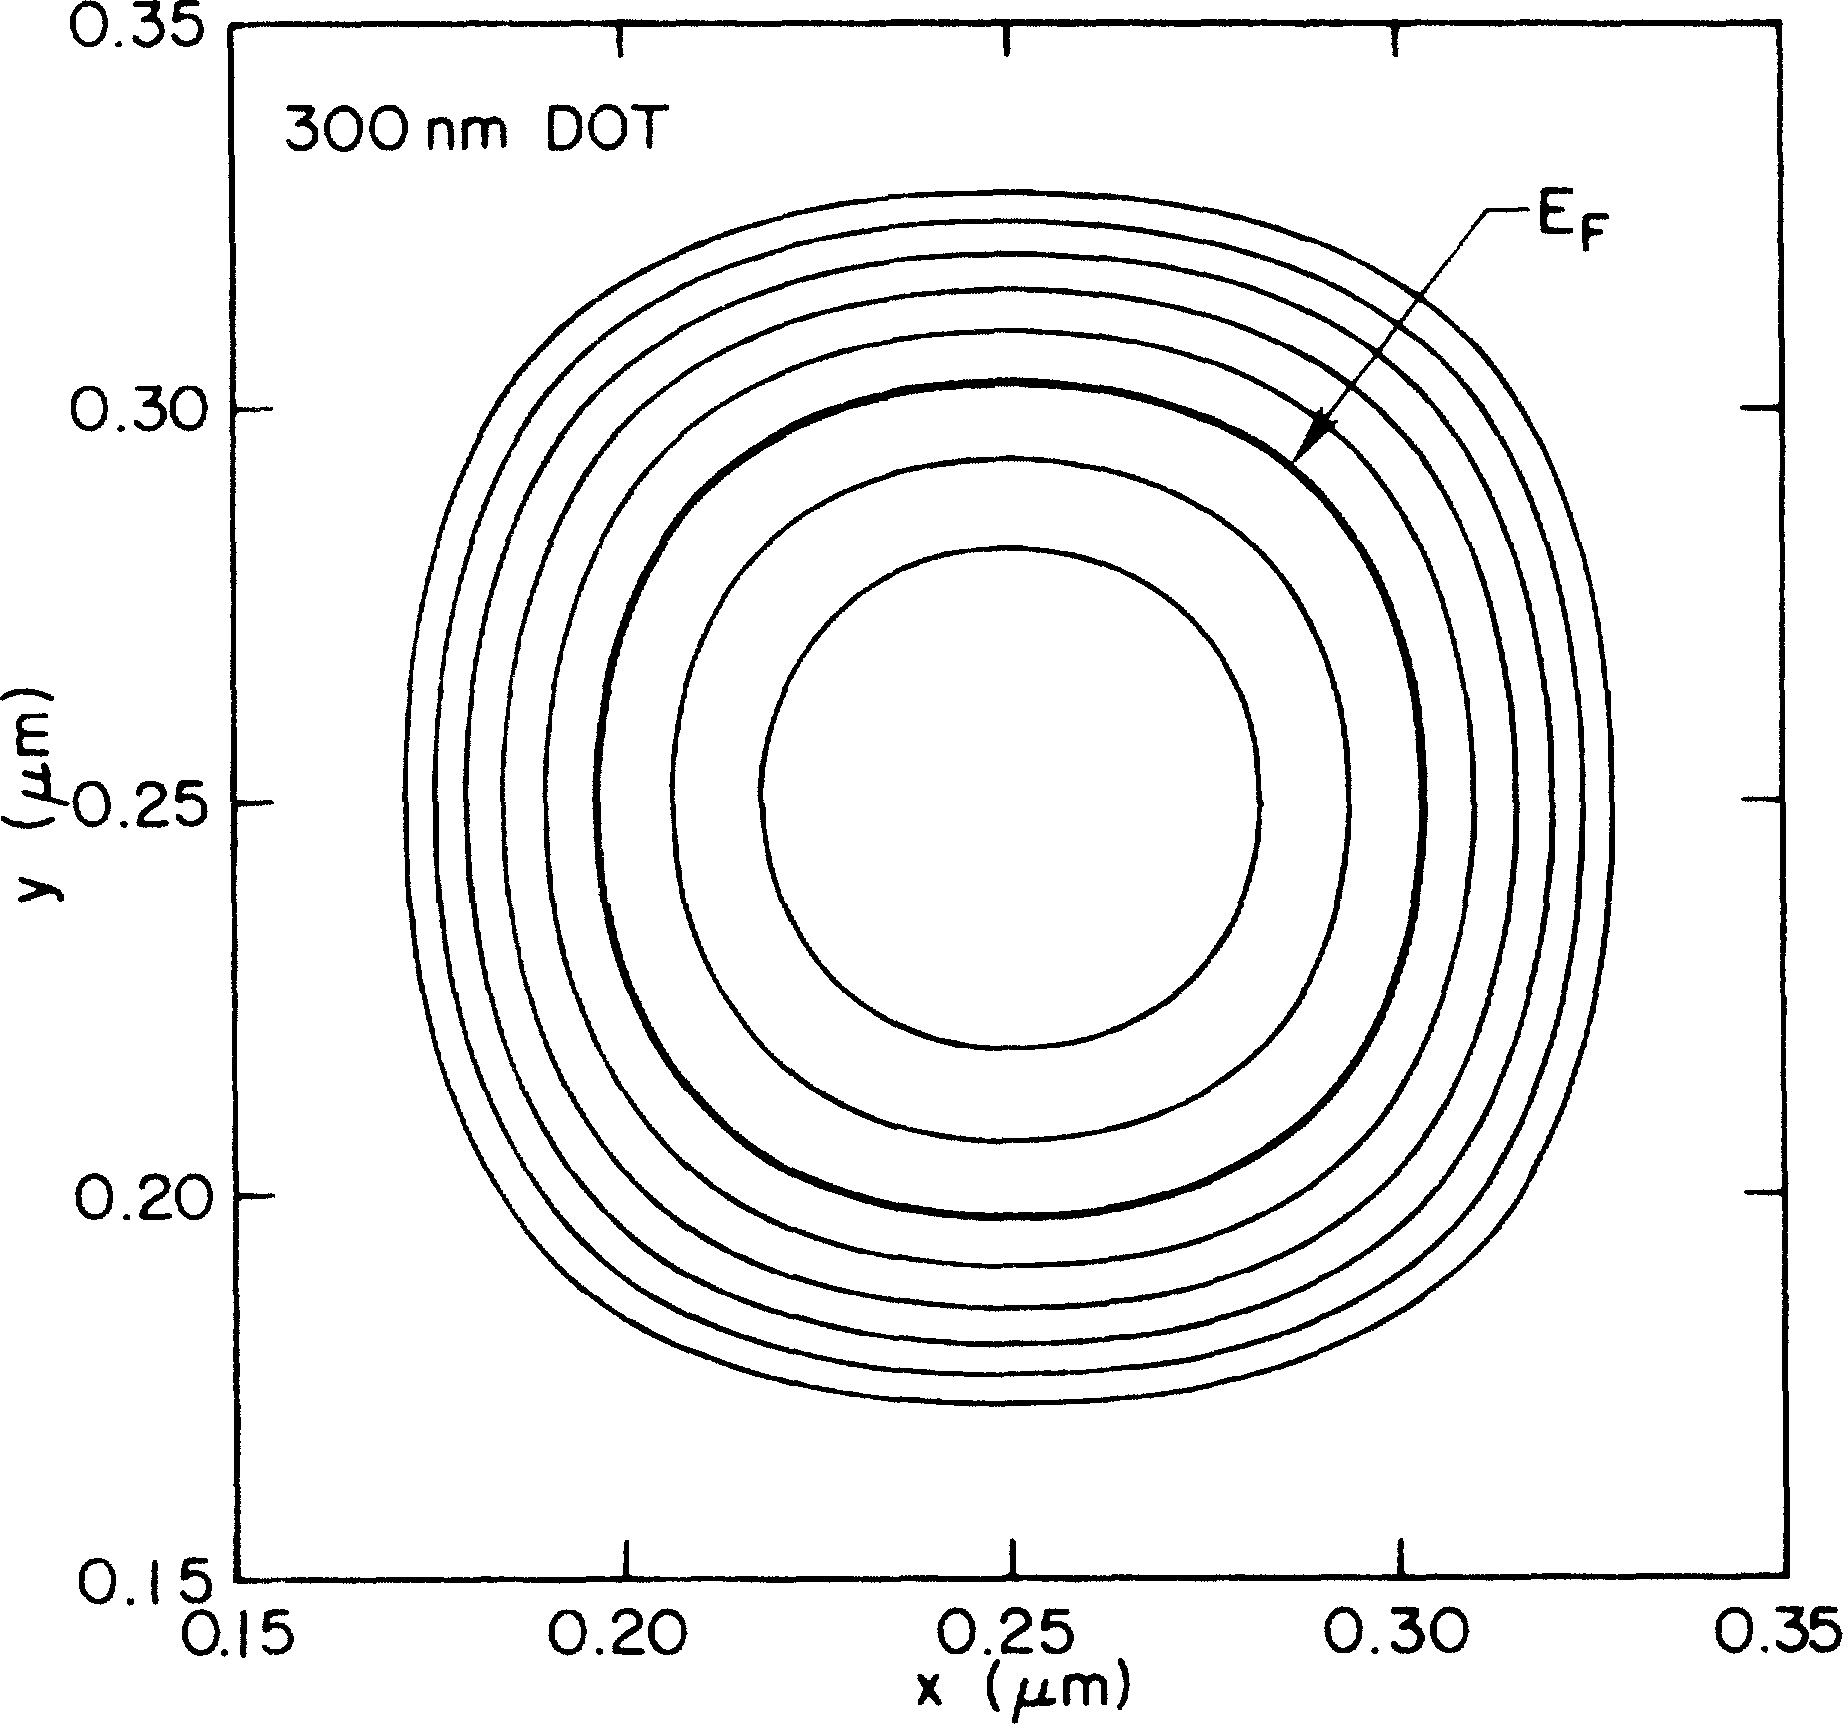
\includegraphics[width=0.55\textwidth]{Figure_2_Kumar}
	\caption{Contours of the lateral potential in a GaAs/AlGaAs quantum dot. The measurements were taken $\SI{8}{\milli\meter}$ below the contact surface of the two materials, and the contours are evenly separated by $\SI{10}{\milli e\volt}$ intervals. The Fermi level (thick line) is indicated by $E_F$. From \cite{Kumar1990}.}
	\label{fig:Figure_2_Kumar}
\end{figure}

An experimental support for this model comes from the observation of far-infrared absorbption spectra, in combination with the Kohn theorem. This theorem \citep[see][]{Kohn1961} states that, for an electron gas with short-range interactions, the latter don't change the cyclotron frequency. For far-infrared absorbption measurements in a quantum dot, this has the consequence that the effects of the electron-electron interaction show up only for a strong enough anharmonicity of the confining potential \citep[see][]{Reimann2002}. Since in many measurements the effects of the electron-electron interaction were not seen, the model of a harmonic confinement gained ground.

We also showed, in sections \ref{sec:shell_model}-\ref{sec:shell_model_evidences}, that a 2D harmonic oscillator gives the same magic numbers observed experimentally. An improved model, that takes into account the non-zero thickness of a lateral dot (neglected for a pure 2D potential), would be to add a $z$-contribution to the potential, i.e. $V=V(x,y,z) = V(x,y) + V(z)$. Then, it is assumed that the only state occupying the $z$-direction is the ground state, so that the solution can be restricted to the $(x,y)$-plane \citep[see][]{Reimann2002}. $V(x,y)$ is modeled as the usual two-dimensional parabolic confinement:
\begin{equation}
	V(x,y)=\frac{1}{2}m\omega^2(x^2+y^2)
\end{equation}

It's worth noting that, in experimental observations, the effective confinement strength $\omega$ is not constant; it tends to lower as the number $N$ of confined electrons increases. The lowering of the effective strength translates into an increase of the ``confinement volume'', so that the electron density remains constant. A model for $\omega$ that takes into account these effects was given by \cite{Koskinen1997}, who modeled $\omega^2$ as
\begin{equation}
	\omega^2 = \frac{e^2}{4\pi\varepsilon m^*r_s^3\sqrt{N}},
\end{equation}
where $\varepsilon$ is the dielectric constant of the material, $m^*$ is the effective mass of the electron and $r_s$ is the average electron-density parameter\footnote{
	This parameter is also called the \emph{Wigner-Seitz} parameter. It's defined such that
	\begin{equation*}
		\Omega_d(r_s) = n,
	\end{equation*}
	where $\Omega_d(r_s)$ is the spherical volume of radius $r_s$ in $d$ dimensions (e.g., for $d=2$ is a circle with radius $r_s$) and $n$ is the mean volume per unit electron (i.e., the mean electron density). So, $r_s$ can be expressed as
	\begin{equation*}
		r_s = \frac{1}{\sqrt{\pi n}}
	\end{equation*}
	for the two-dimensional case, or as
	\begin{equation*}
		r_s = \left(\frac{3}{4\pi n}\right)^{1/3}
	\end{equation*}
	for the three-dimensional case.
},
quite close to the equilibrium value  for a two-dimensional electron gas \citep[see][]{Reimann2002}.
